%%%%%%%%%%%%%%%%%%%%%%%%%%%%%%%%%%%%%%%%%
% Visualization and Visual Data Analysis
%
% Author:
% Benjamin Neckam
% Alexander Gelb
% Nicole Cherches
% Axinya Tokareva
%
%%%%%%%%%%%%%%%%%%%%%%%%%%%%%%%%%%%%%%%%%

\documentclass{article}

\usepackage[utf8]{inputenc}
\usepackage{textcomp}
\usepackage{graphicx}
\usepackage{url}

\begin{document}
\title{Visualization and Visual Data Analysis}
\author{Nicole Cherches, Alexander Gelb, Benjamin Neckam, Axinya Tokareva}
\maketitle
\section{M2 - Lo-Fi Prototyping}
\subsection{Proposed visualization solution}
The user interface is oriented on programs like "Tableau" or "Glue" because we think it is the most easiest and most intuitive way to work with data. Figure 1 shows a very rough prototype of it with just two main parts:\\
\begin{itemize}
\item Information view
\item Plot view
\end{itemize}

\begin{figure}[!h]
\centering
    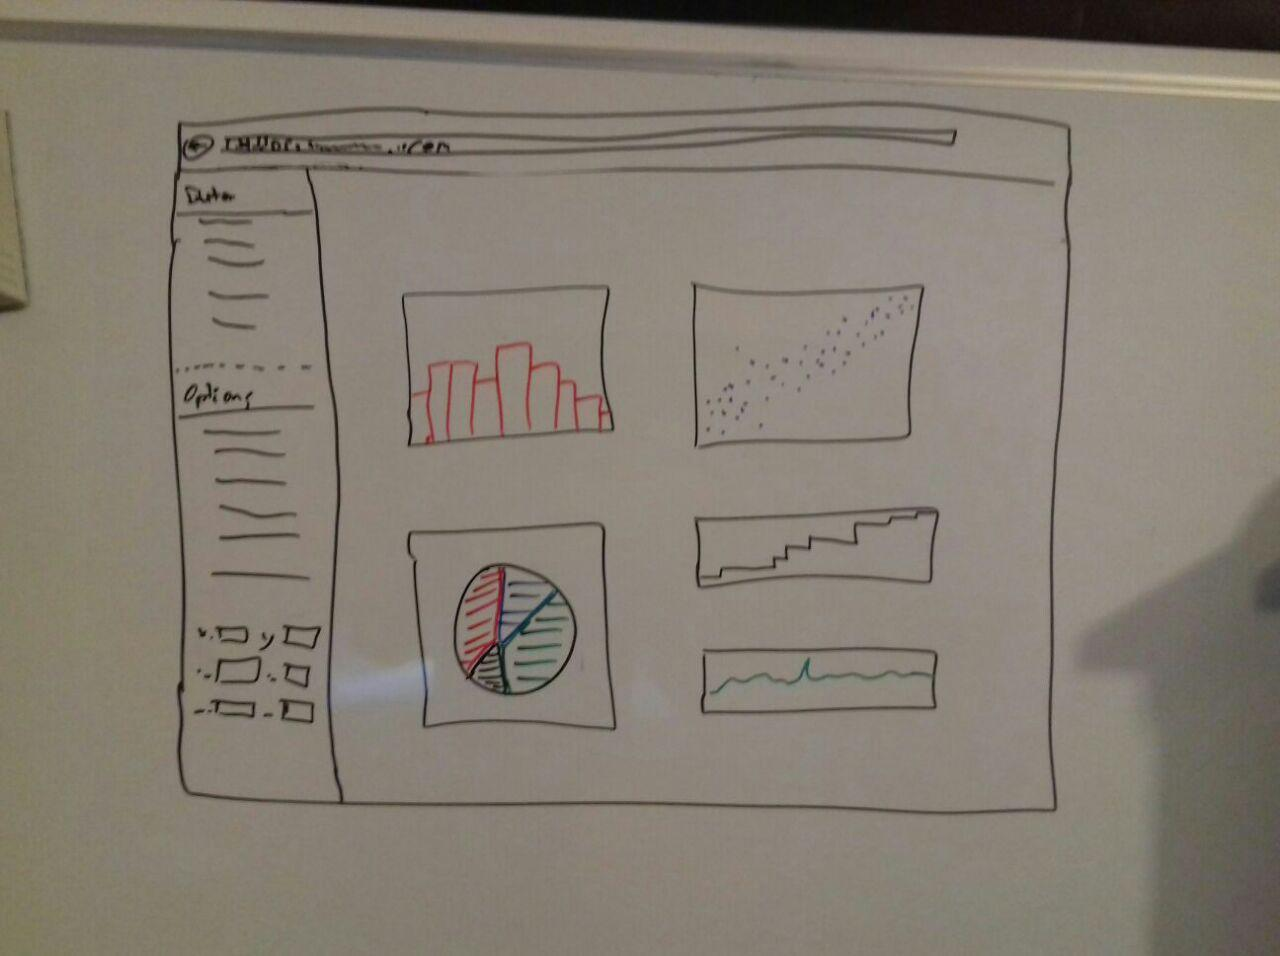
\includegraphics[width=0.75\textwidth]{images/Prototype1.jpg}
	\caption{User interface}
	\label{fig1}
\end{figure}

\subsubsection{Information view}
At the moment the information view, figure 2, is divided in two parts, "Data" and "Options". Data provides some information about the dataset itself like name of the table, number of columns, rows and entries or column names. Options should give the possibility to add plots, interactions and other things to the plot view.
\begin{figure}[!h]
\centering
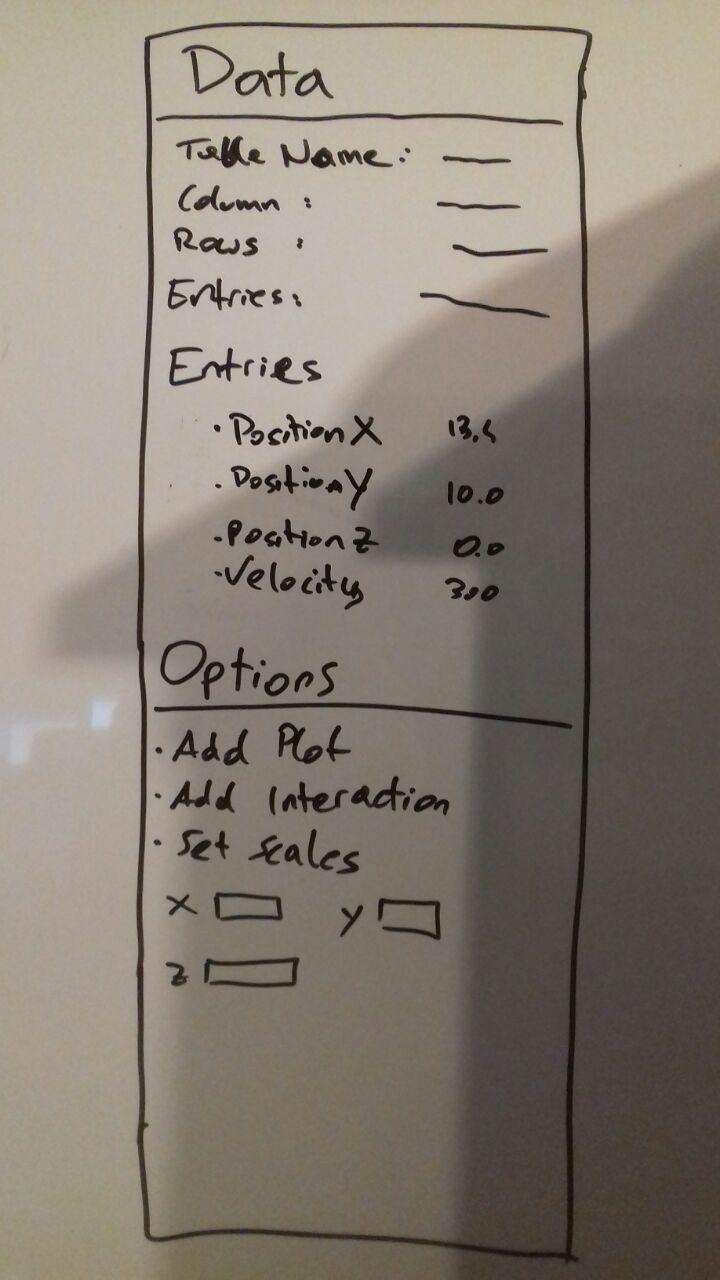
\includegraphics[width=0.3\textwidth]{images/InformationView.jpg}
	\caption{Information view}
	\label{fig2}
\end{figure}
\subsubsection{Plot view}
The plot view is the area where, like the name tells us, all the plots appear and the interaction happens.
\subsubsection{Graph proposals}
Since we did not get a real specification of the customer what he would like to get visualize and just told us to try out whatever we want, we came up with a few ideas which might be interesting for astronomers. Unfortunately there are just 4 things, distance to sun, color, position and amount of stars which can be plotted in a meaningful manner, which made it really hard to find good plotting examples. At least we got six ideas so far and hope that the process of working with the data more intense we get new ideas for new plots.
\begin{itemize}
\item Scatterplot which shows the number of stars compared to the distance of the sun. (figure 3)\\
\\
Advantage is to get a good overview of how the stars are distributed in the area around the sun.
An disadvantage will be the confusion if there are to many stars and therefore no chance to find any patterns or other interesting things.
\begin{figure}[!h]
\centering
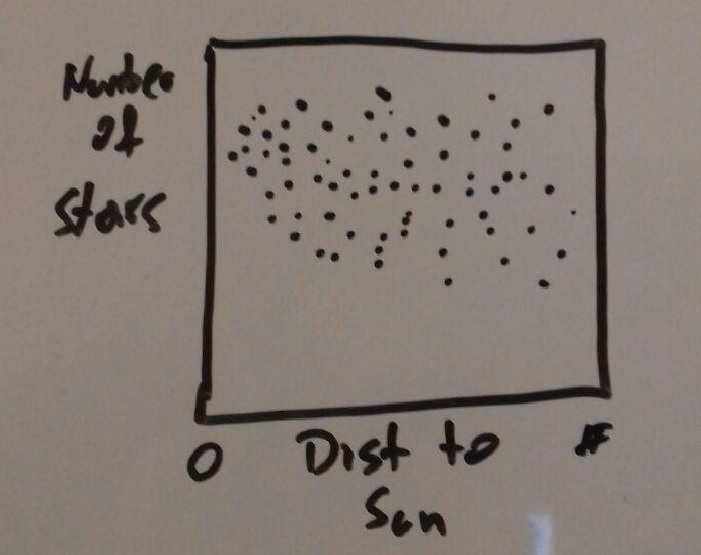
\includegraphics[width=0.5\textwidth]{images/NumbStarsDistSun.jpg}
	\caption{Scatterplot}
	\label{fig3}
\end{figure}
\item 3D representation of star clusters around the sun. (figure 4)\\
\\
Since the universe is a three dimensional space it is easier to see where specific star clusters are located but we are not sure if it is possible to create such a visualization with D3.
\begin{figure}[!h]
\centering
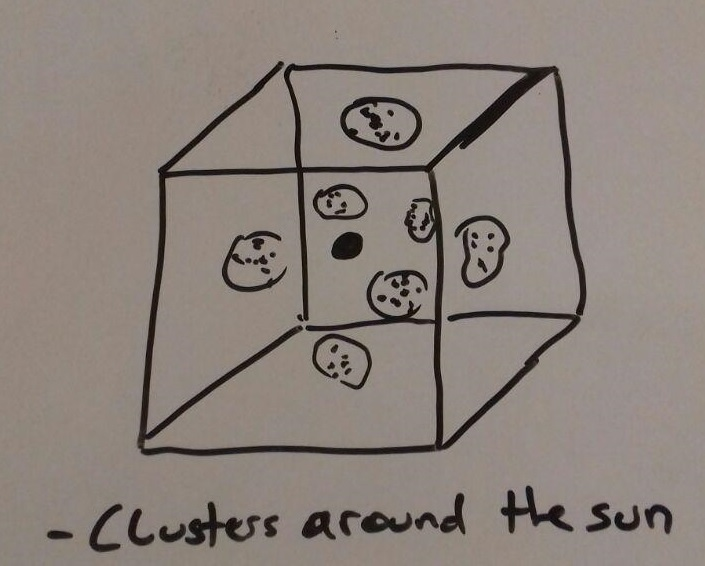
\includegraphics[width=0.5\textwidth]{images/ClustersSun3d.jpg}
	\caption{3D visualization}
	\label{fig4}
\end{figure}
\item The ratio of hot and cold stars. (figure 5)\\
\\
It is very easy to understand but it can give a wrong picture of the data since not all stars has the state of their temperature.
\begin{figure}[!h]
\centering
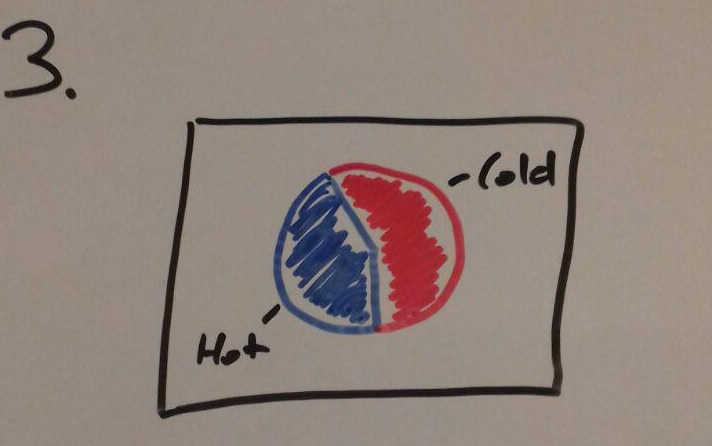
\includegraphics[width=0.5\textwidth]{images/HotColdRatio.jpg}
	\caption{Pie chart}
	\label{fig5}
\end{figure}
\newpage\item Bar chart showing the size of specific star clusters. (figure 6)\\
\\
Like the pie it is very self explaining but if for example the scale of the y-axis is chosen wrong at can lead to false interpretation.
\begin{figure}[!h]
\centering
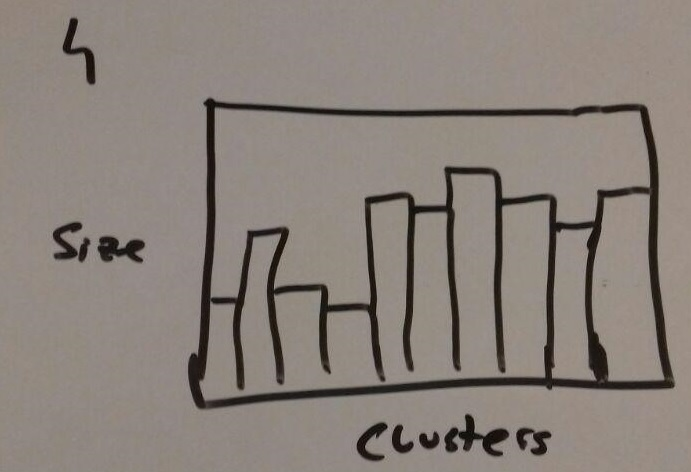
\includegraphics[width=0.5\textwidth]{images/SizeClusters.jpg}
	\caption{Bar diagram}
	\label{fig6}
\end{figure}
\item Line graph showing how the velocity behaves to the distance to the sun. (figure 7)\\
\\
An advantage of this view is that it shows in a good way of how the velocity changes with the distance to the sun but like with the bar chart choosing a good scale for the axis is important.

\begin{figure}[!h]
\centering
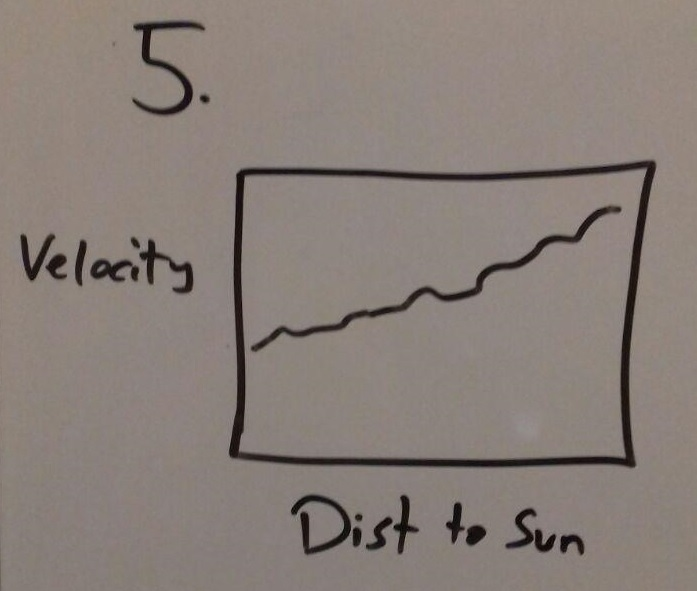
\includegraphics[width=0.5\textwidth]{images/VelocityDist.jpg}
	\caption{Line graph}
	\label{fig7}
\end{figure}
\newpage\item Shows the movement of a star in a certain time. (figure 8)\\
\\
Good could be to see if a star is moving and how much it is moving in terms of time.
Disadvantage is that it is hard to compare many stars and how they are moving, because it just will show the motion of one star.

\begin{figure}[!h]
\centering
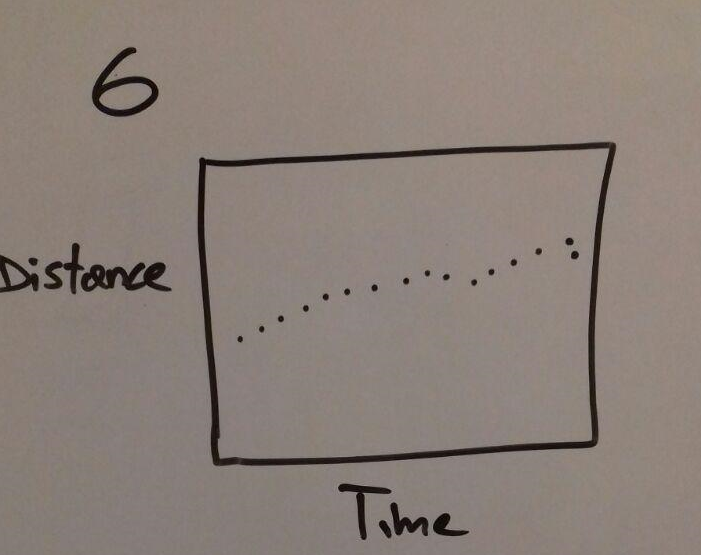
\includegraphics[width=0.5\textwidth]{images/DistanceTime.jpg}
	\caption{Dot plot}
	\label{fig8}
\end{figure}
\item Shows if there is a correlation in the parallax and the proper motion of the stars. (figure 9)\\
\\
The scatter plot could show the correlation if there is one but it is also possible that the amount of data makes it impossible to find out if a correlation exists. 
\begin{figure}[!h]
\centering
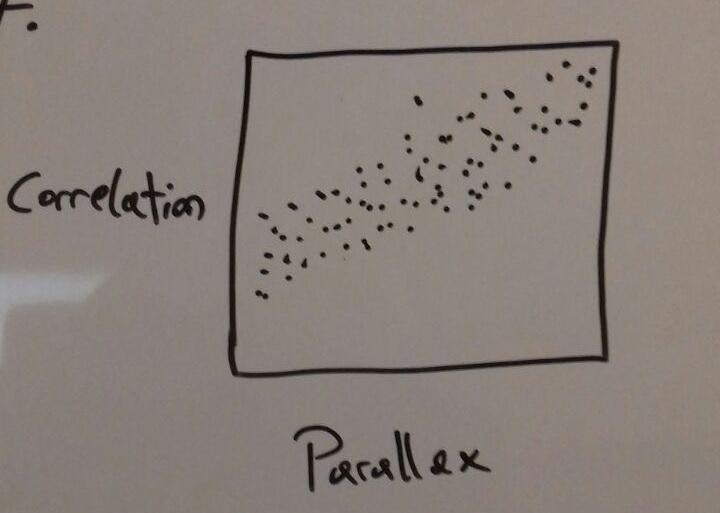
\includegraphics[width=0.5\textwidth]{images/CorrelationParallax.jpg}
	\caption{Scatter plot }
	\label{fig9}
\end{figure}
\newpage \item The Boxplot should show the minimum, maximum, average and median of errors of a specific star cluster. (figure 10)\\
\\
It can give a good overview of how the errors of measurement are distributed inside the star cluster. A disadvantage is that the data are potentially not meaningful because maybe some stars has no error measures and so the plot is corrupted.
\begin{figure}[!h]
\centering
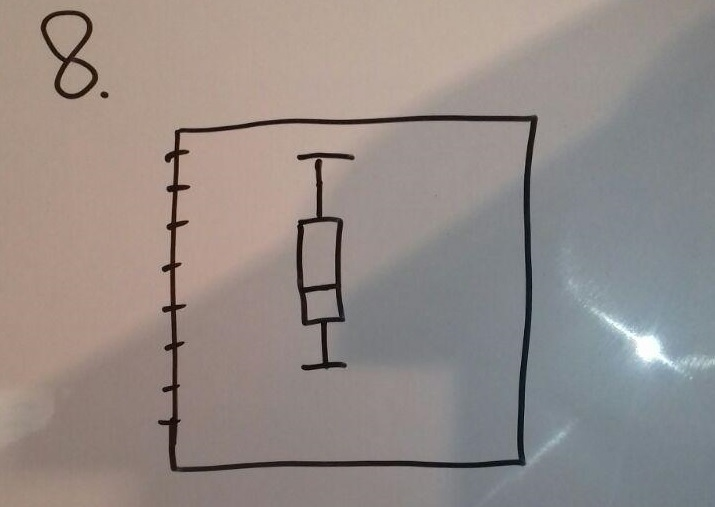
\includegraphics[width=0.5\textwidth]{images/Boxplot.jpg}
	\caption{Boxplot }
	\label{fig10}
\end{figure}
\item To show how the measured error behaves in comparison to the velocity a line graph will be used. (figure 11)\\
\\
Advantage is it shows if the velocity has an influence on the error of the stars. Possible disadvantage is that the plot is not meaningful.
\begin{figure}[!h]
\centering
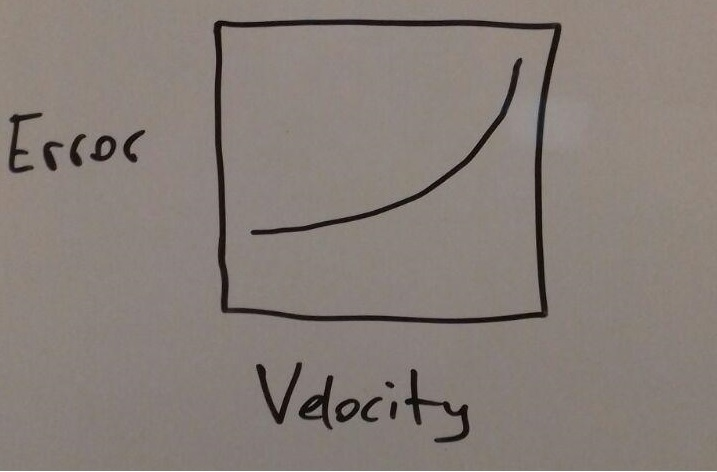
\includegraphics[width=0.5\textwidth]{images/VelocityError.jpg}
	\caption{Linegraph  }
	\label{fig11}
\end{figure}
\newpage\item The plot should compare the different types of weights, AC and AL (when writing this, we have not received an answer of the experts yet what it is exactly, but we thought it could be interesting), inside a star cluster. (figure 12)\\
\\
Can give a good comparison of the two different weight types, but since we don't know what it exactly is yet we can not really say if it is a good and useful representation.
\begin{figure}[!h]
\centering
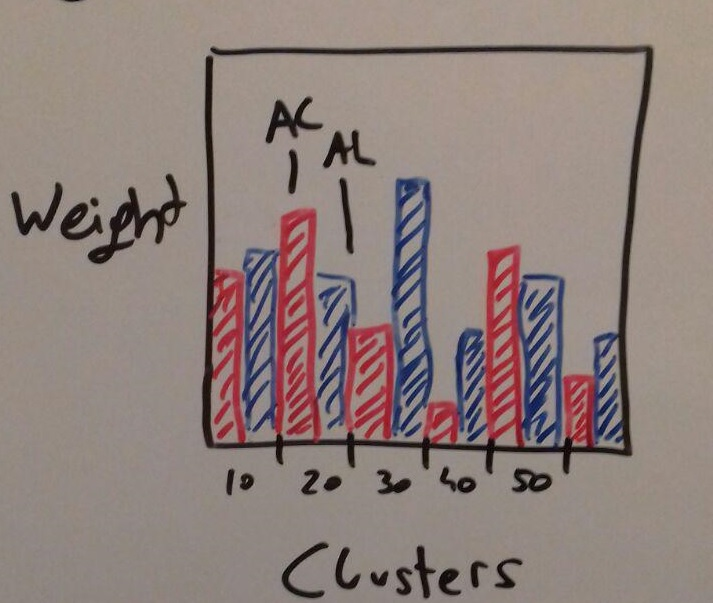
\includegraphics[width=0.5\textwidth]{images/ClustersWeight.jpg}
	\caption{Bargraph  }
	\label{fig12}
\end{figure}
\end{itemize}

\newpage

\subsubsection{Interactions}
\begin{enumerate}
\item \textbf{Dashboard 1} \\
One dashboard could be to combine figure 4, 5, 6 and 12. While figure 4 shows the star clusters around the sun in a three dimensional context, figure 5 can give us an overview of the ratio of hot and cold stars in the data. To see how many stars are inside of a cluster, figure 5 can provide the information with a bar chart. Figure 12 contains the two types of weight of each cluster and compares the cumulated weights. The interactions could be to click on a specific cluster in the three dimensional representation and figure 5 and 6 updates their values corresponding to the selected cluster, while figure 12 highlights the bars of the selected cluster. Another interaction will be when you just want to see all the hot stars, you can select them in figure 5 and all other plots updates their view to show only the hot ones. \\

\textbf{Advantage} \\
With this dashboard it is very easy for the user to recognize patterns (e.g. amount of cold/warm stars in cluster, size of cluster, overall weight of stars in cluster) inside of to the clusters. The user can interact with this dashboard to gain more knowledge for each cluster in an easy and intuitive way. \\

\textbf{Disadvantage} \\
A big disadvantage of this dashboard is the generalization of the stars into clusters. The generalization leads to just see an overall information of the amount of stars and will not provide any information of a specific star. \\

\item \textbf{Dashboard 2} \\
The second idea is to combine figure 4, 7 and 10. As mentioned before, figure 4 shows the clusters around the sun in a 3D scatterplot. Figure 7 plots a line graph sorted by the distance to sun for every star and compares it to the velocity of a star. The last figure (figure 10) plots a box plot of the astronomic excess noise significance of all stars. If a cluster of figure 4 is selected, figure 7 and 10 will plot the line graph and the box plot just according to the stars contained in the chosen cluster. \\

\textbf{Advantage} \\
See if and how the distance to sun changes the velocity of the stars or star clusters and how big the astronomic excess noise significance is. It can be used to see if the error grows with distance and velocity.

\textbf{Disadvantage} \\
It will be very time consuming to process and sort the data every time if an interaction happens. Furthermore many information can be lost in the single views because not all single stars has all needed data and therefore the box plot is not completely true for example.

\item \textbf{Dashboard 3 - Name} \\
2 (sterne), 6, 7, 9
The last dashboard shows figure 4, 8, 9, and 11. Figure 4 plots all stars in a 3D scatterplot in which the user can zoom in and out to get a better sight of the stars. Figure 8 plots the movement of a star in a certain time compared to the distance of this star. For this plot there will be used a 2D scatterplot with brushing and linking to have a clearer view of the data. Figure 9 shows also a 2D scatterplot with brushing and linking with the distance to the sun of each star compared to the correlation of the distance to the sun and movement of a star. The last figure plots the error of velocity compared to velocity of each star as a simple line graph. One interaction will be the tooltip technique in figure 4. If a star is clicked in the 3D scatterplot, there will popup a tooltip with useful informations about this star. Furthermore the movement of the star will be plotted in figure 8. Another way to select a star for figure 8 will be to click a star in figure 7, which will also lead to zoom in to the chosen star in figure 4. \\

\textbf{Advantage} \\
The big advantage of this dashboard is, that the user is able to gain information and interesting patterns about specific stars and not only a whole cluster. \\

\textbf{Disadvantage} \\
The disadvantage can be that the user will be overwhelmed of the amount of data and is not able to extract useful information of for example figure 9.  \\

\end{enumerate}

\subsubsection{VIS Techniques}
\begin{itemize}
\item \textbf{Zoom} \\
Because of the big amount of data, the zoom technique is very important for the stars around the sun and clusters around the sun 3D scatterplot. With the billions of stars in a dataset the plot has so many dots (stars) in it, that the user wouldn't be able to extract relevant information of the plot. The user should be able to zoom in and out of the Scatterplot and turn the plot around to get another sights of the distribution and information of stars and clusters.

\item \textbf{Tooltip} \\
Combined with the zoom function, the tooltip technique shows special information of a dot (e.g. name of the star, weight, distance to sun,...) if a star/cluster is clicked. This can be very useful if a dot attracts the attention of the user because of a strange behaviour (e.g. bunch of stars in a close area).

\item \textbf{Brushing and Linking} \\
The brushing and linking will be very helpful for the user to set limits to the min and max value of a scatterplot. For the 2D scatterplots there we have the same problem as with the 3D scatterplot. Because of the amount of data the user will be overwhelmed of the information and won't be able to extract useful information of the plot. With the brushing and linking technique the user can decide on his own what minimum and maximum is interesting to see for him and so can also just have a look on small parts of the data.

\item \textbf{Filter} \\
For all of the plots we will need filters to filter useless data which will have no values, null values or other values we could not process.

\item \textbf{Dimension Stacking} \\
The dimension stacking is used for the mean astronomic weight of the source in AL and AC direction compared to each cluster. The user has a fast overview of both weight variables for each cluster, which is triggers an interaction with other plots if clicked. This can help to determine eyecatching information of special clusters very fast.
\end{itemize}

\end{document}